\subsubsection{Run Session}
\begin{figure}[H]
    \centering
    \begin{subfigure}{\linewidth}
        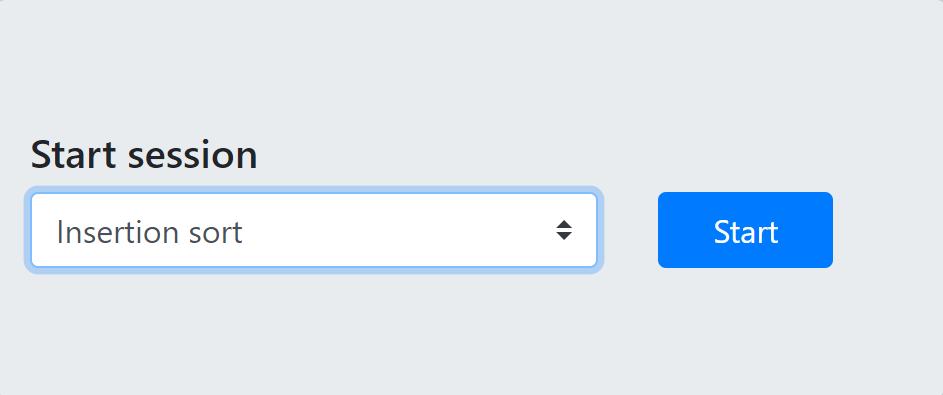
\includegraphics[width=\linewidth]{/userManual/admin/selectSessionToRun}
       	\caption{}
		\label{fig:RunSessionOverview}	
    \end{subfigure}
\end{figure}
Using figure: \ref{fig:RunSessionOverview}
\begin{userManualItemlist}
    \item[Step I.] Navigate to the Admin page.
    \item[Step II.] Select a session from the list.
    \item[Step III.] Click the "Start" button.
\end{userManualItemlist}

\begin{figure}[H]
    \centering
    \begin{subfigure}{\linewidth}
        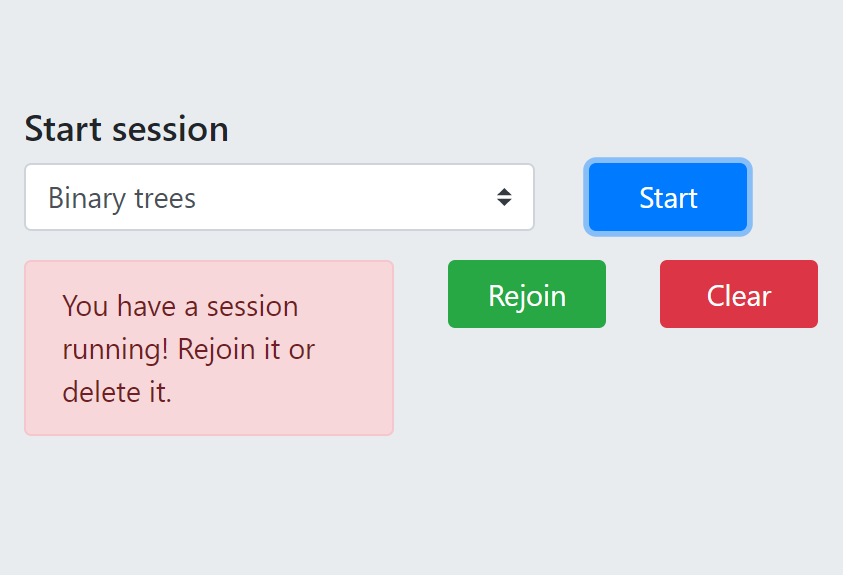
\includegraphics[width=\linewidth]{/userManual/admin/selectSessionToRunError}
       	\caption{}
		\label{fig:RunSessionOverviewError}	
    \end{subfigure}
\end{figure}
\begin{minipage}{0.45\linewidth}
    \subsubsection{Rejoin an active session}
    \begin{userManualItemlist}
        \item[Step I.] Click the "Rejoin" button. (Figure: \ref{fig:RunSessionOverviewError})
    \end{userManualItemlist}
\end{minipage}
\hfill
\begin{minipage}{0.45\linewidth}
    \subsubsection{Clear an active session}
    \begin{userManualItemlist}
        \item[Step I.] Click the "clear" button. (Figure: \ref{fig:RunSessionOverviewError})
    \end{userManualItemlist}
\end{minipage}


\subsubsection{Waiting Room}
\begin{figure}[H]
    \centering
    \begin{subfigure}{\linewidth}
        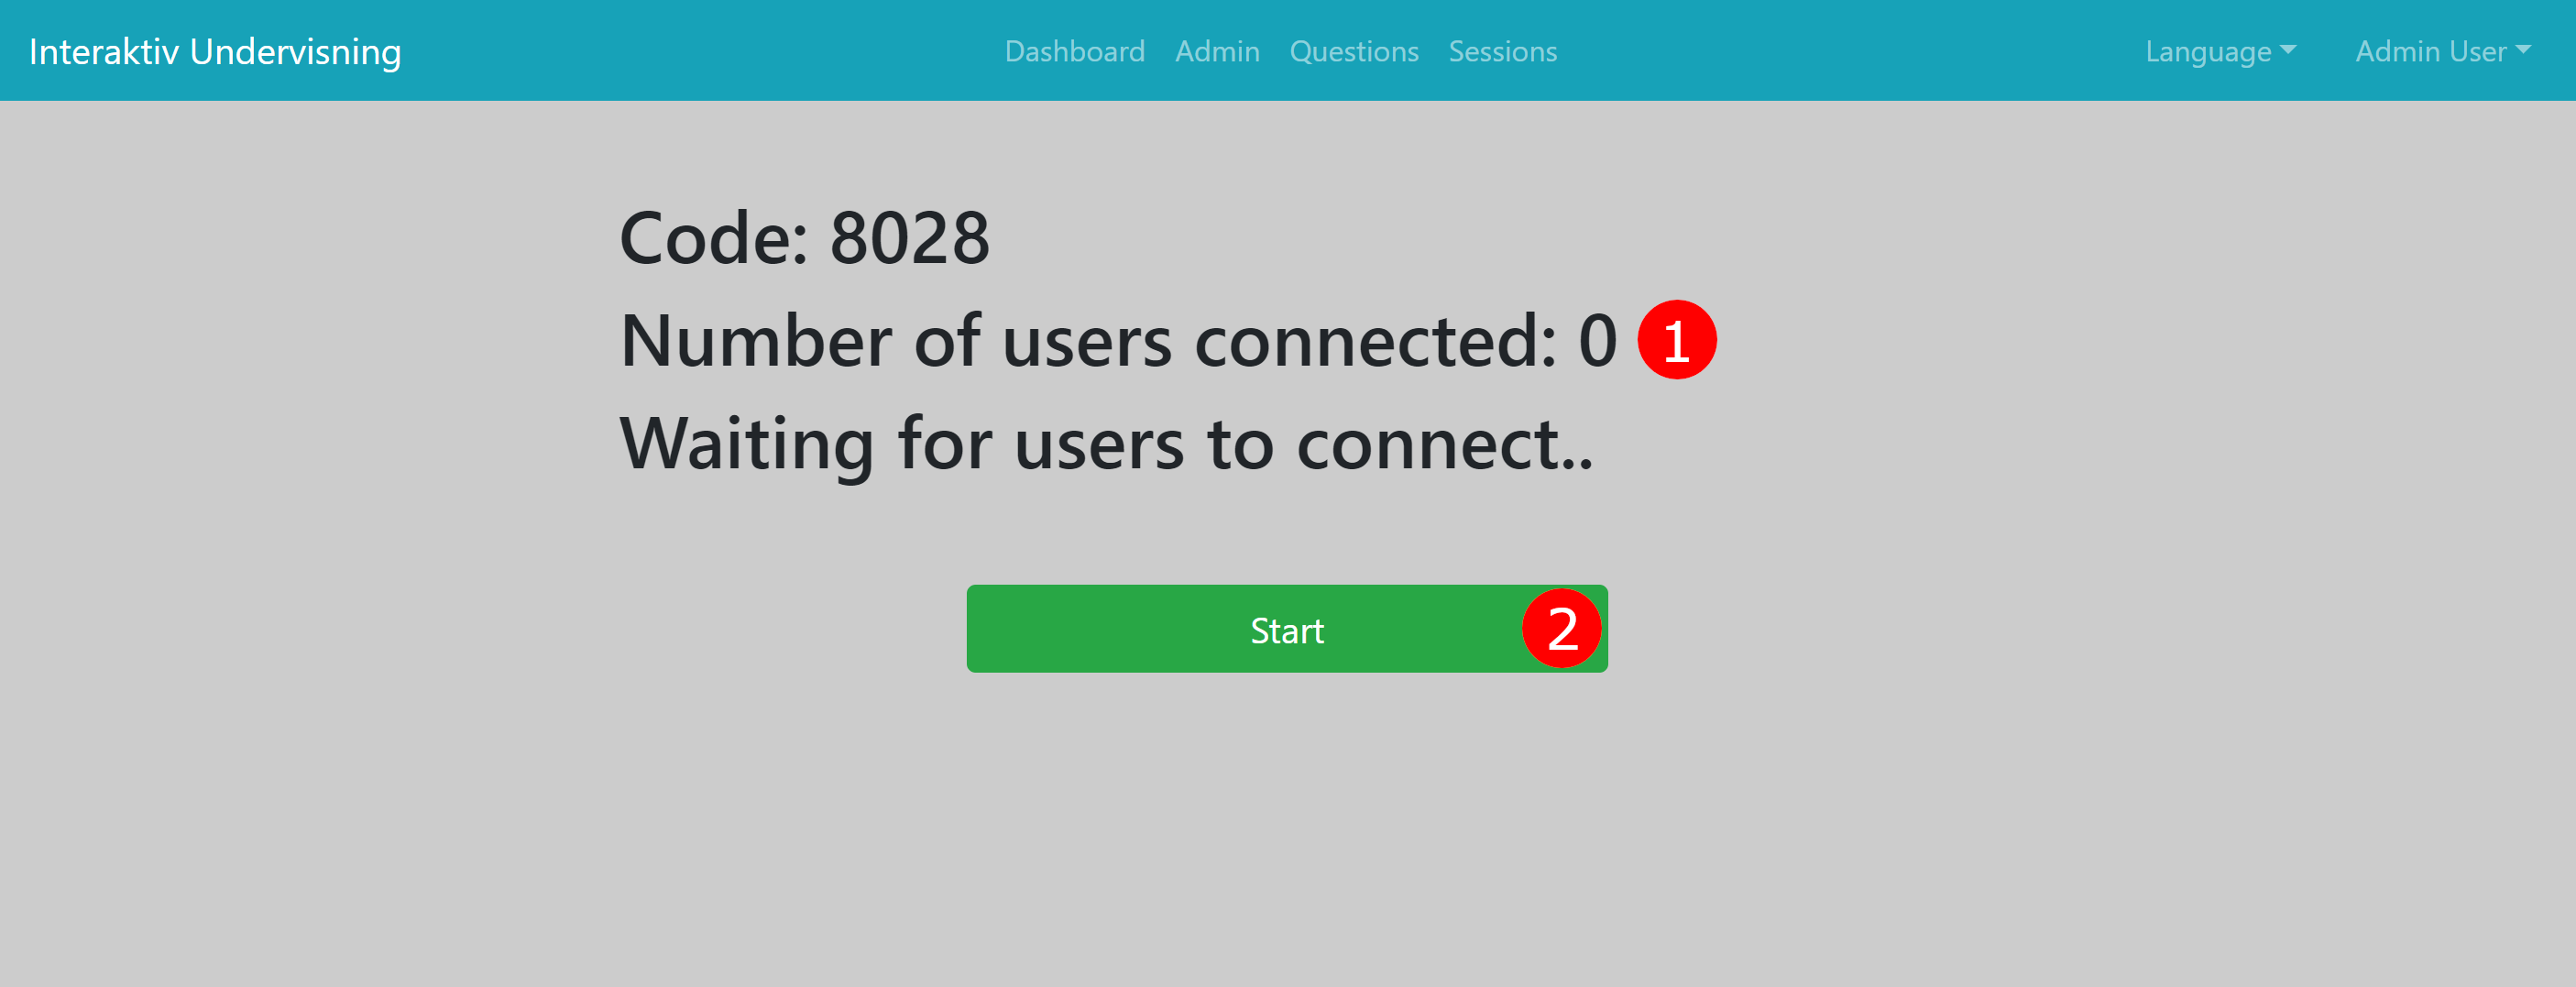
\includegraphics[width=\linewidth]{/userManual/admin/activeSessionWaitingRoom}
       	\caption{}
		\label{fig:activeSessionWaitingRoom}	
    \end{subfigure}
\end{figure}
Using figure: \ref{fig:activeSessionWaitingRoom}
\begin{userManualItemlist}
    \item[1] Shows the currently connected number of participants.
    \item[2] If there are more than zero participants, this button starts the session.
\end{userManualItemlist}

\subsubsection{During a Question}
\begin{figure}[H]
    \centering
    \begin{subfigure}{\linewidth}
        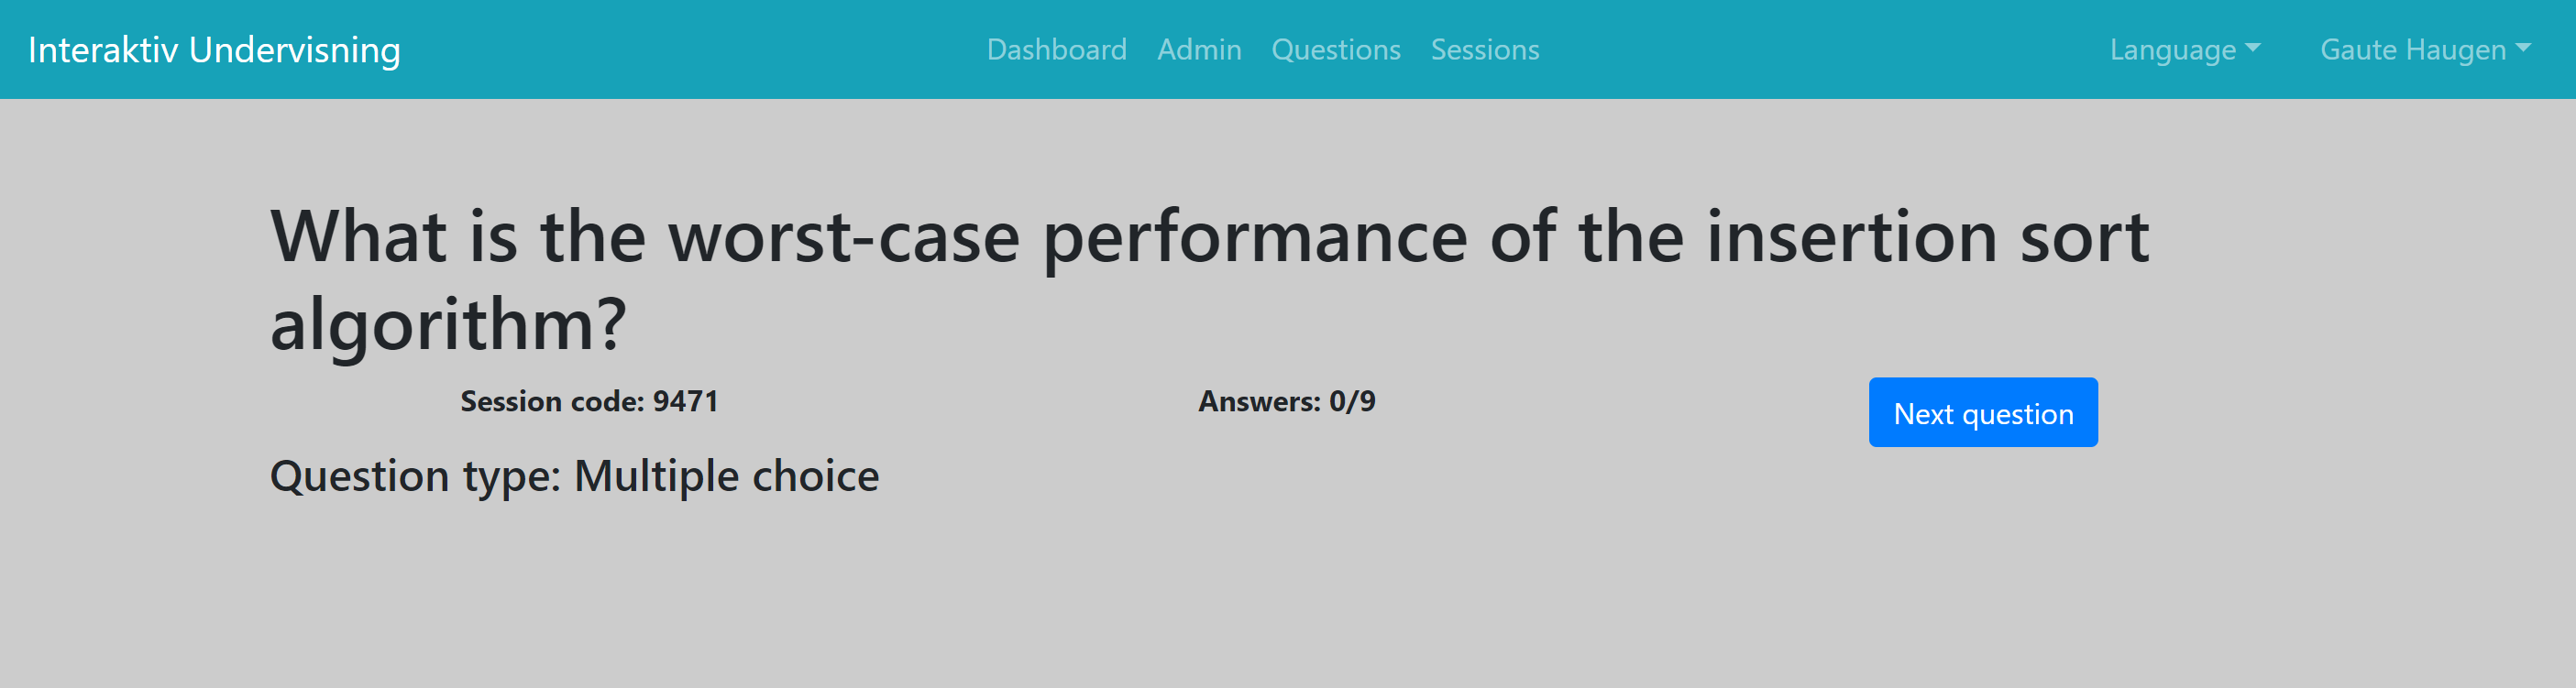
\includegraphics[width=\linewidth]{/userManual/admin/activeSessionQuestion}
       	\caption{}
		\label{fig:activeSessionQuestion}	
    \end{subfigure}
\end{figure}
Using figure: \ref{fig:activeSessionQuestion}
\begin{userManualItemlist}
    \item[1] Is the current session code users can use to join.
    \item[2] Is showing how many students have answered the question.
    \item[3] This button forces the next question.  
\end{userManualItemlist}

\subsubsection{During the Result Screen}
\begin{figure}[H]
    \centering
    \begin{subfigure}{\linewidth}
        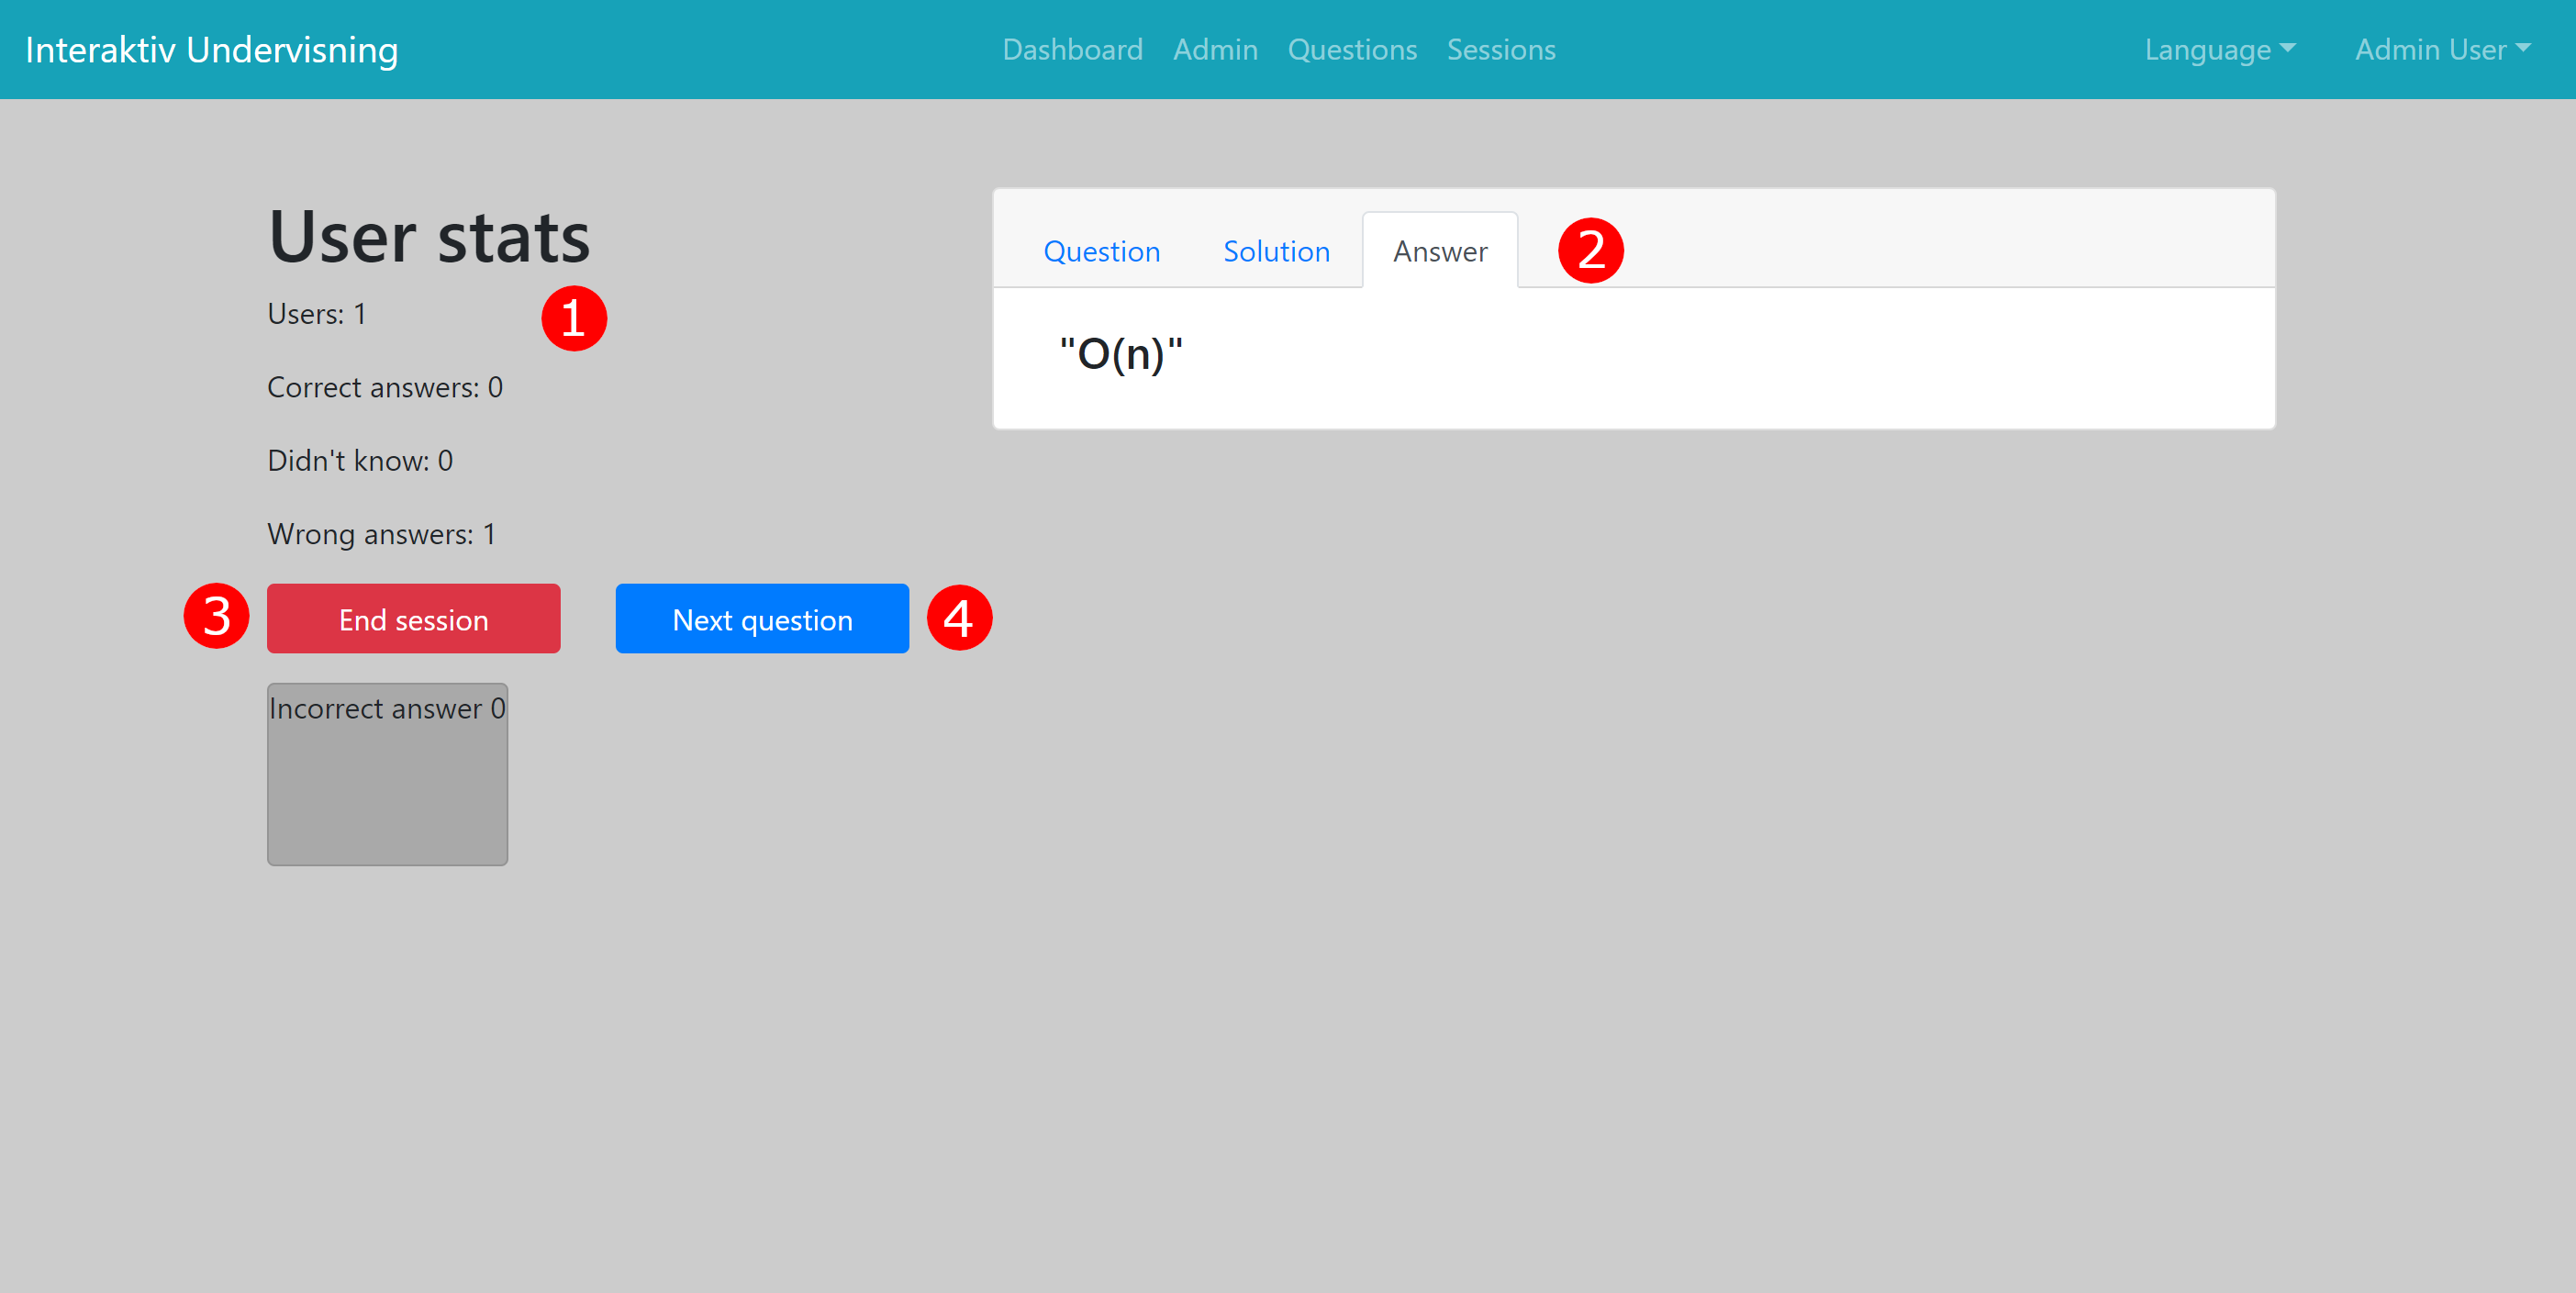
\includegraphics[width=\linewidth]{/userManual/admin/activeSessionResultScreen}
       	\caption{}
		\label{fig:activeSessionResultScreen}	
    \end{subfigure}
\end{figure}
Using figure: \ref{fig:activeSessionResultScreen}
\begin{userManualItemlist}
    \item[1] This area shows statistics about the question.
    \item[2] This area shows the question information, the solution, and the currently selected wrong answer.
    \item[3] This button can be used by the host to leave the session. The session is still active for 5 minutes.
    \item[4] This button moves the session on to the next question  
\end{userManualItemlist}

\subsubsection{When the Session is Over}
\begin{figure}[H]
    \centering
    \begin{subfigure}{\linewidth}
        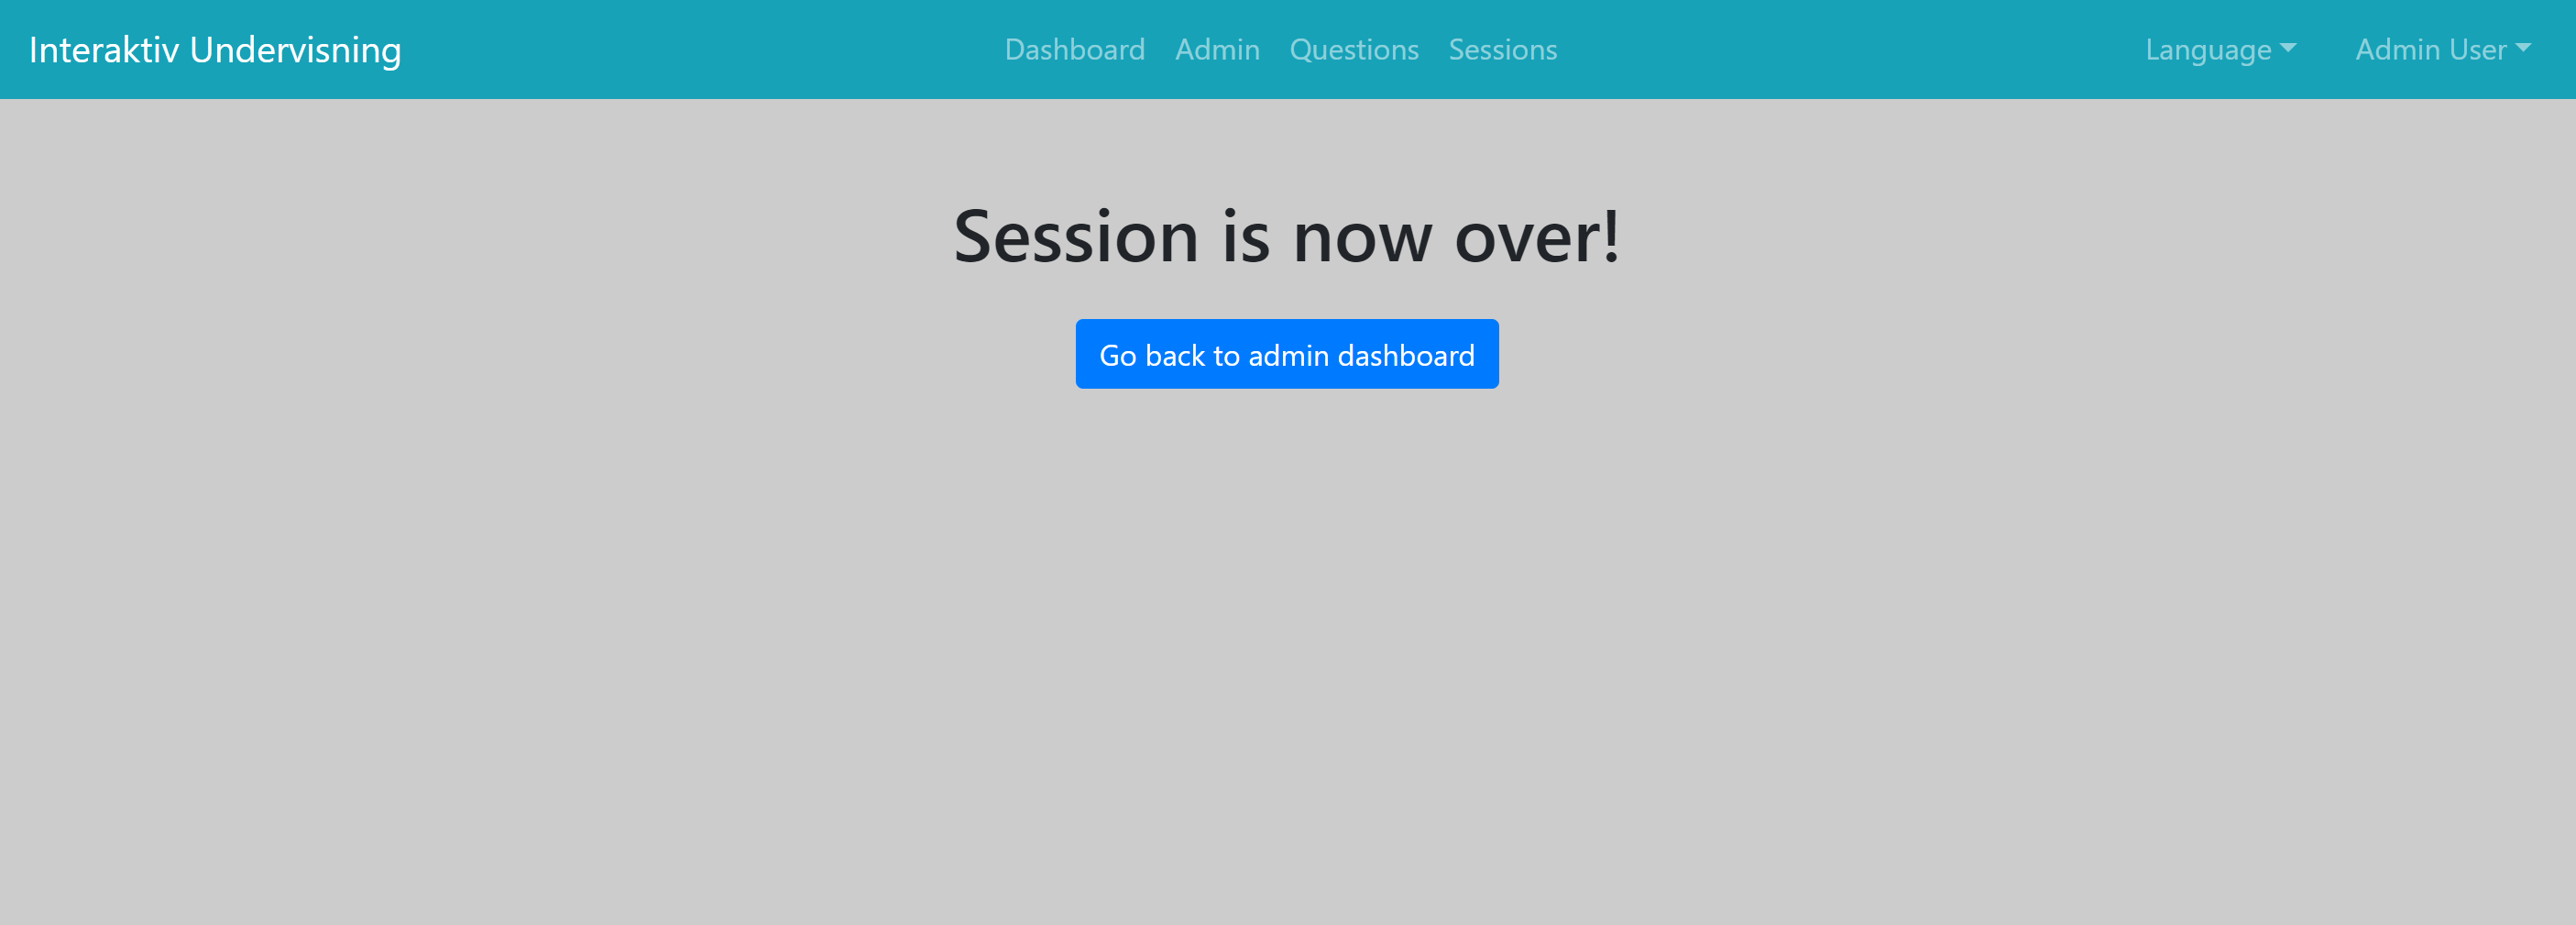
\includegraphics[width=\linewidth]{/userManual/admin/activeSessionOverScreen}
       	\caption{}
		\label{fig:activeSessionOverScreen}	
    \end{subfigure}
\end{figure}
\begin{userManualItemlist}
    \item[1] This button is used to leave the ended session. (Figure: \ref{fig:activeSessionOverScreen})
\end{userManualItemlist}